\section{Yocto Project Resources}

\begin{frame}
  \frametitle{Yocto Project documentation}
  \begin{itemize}
  \item \url{https://docs.yoctoproject.org/}
  \item Wiki: \url{https://wiki.yoctoproject.org/wiki/Main_Page}
  \item \url{https://layers.openembedded.org/}
  \end{itemize}
\end{frame}

\begin{frame}
  \frametitle{Useful Reading (1)}
  \begin{columns}
    \column{0.7\textwidth}
    Embedded Linux Development Using Yocto Project - Third Edition, April 2023
    \begin{itemize}
    \item \url{https://www.packtpub.com/product/embedded-linux-development-using-yocto-project-third-edition}
    \item By Daiane Angolini and Otavio Salvador
    \item From basic to advanced usage, helps writing better, more
      flexible recipes. A good reference to jumpstart your Yocto
      Project development.
    \end{itemize}
    \column{0.3\textwidth}
    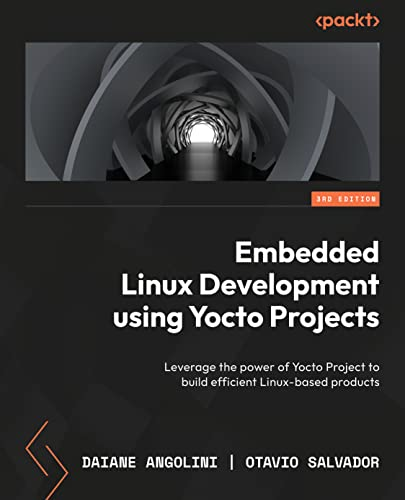
\includegraphics[width=\textwidth]{slides/yocto-resources/ELDYP.jpg}
  \end{columns}
\end{frame}

\begin{frame}
  \frametitle{Useful Reading (2)}
  \begin{columns}
    \column{0.7\textwidth}
    Embedded Linux Projects Using Yocto Project Cookbook - Second Edition, January 2018
    \begin{itemize}
    \item \url{https://www.packtpub.com/virtualization-and-cloud/embedded-linux-development-using-yocto-project-cookbook-second-edition}
    \item By Alex González
    \item A set of recipes that you can refer to and solve your
          immediate problems instead of reading it from cover to cover. 
    \end{itemize}
    See our review: \url{https://bit.ly/1GgVmCB}
    \column{0.3\textwidth}
    \includegraphics[width=\textwidth]{slides/yocto-resources/ELPYPC.jpg}
  \end{columns}
\end{frame}
